\documentclass[
  stu,
  floatsintext,
  longtable,
  a4paper,
  nolmodern,
  notxfonts,
  notimes,
  colorlinks=true,linkcolor=blue,citecolor=blue,urlcolor=blue]{apa7}

\usepackage{amsmath}
\usepackage{amssymb}



\usepackage[bidi=default]{babel}
\babelprovide[main,import]{spanish}
\StartBabelCommands{spanish}{captions} [unicode, fontenc=TU EU1 EU2, charset=utf8] \SetString{\keywordname}{Palabras
Claves}
\EndBabelCommands


% get rid of language-specific shorthands (see #6817):
\let\LanguageShortHands\languageshorthands
\def\languageshorthands#1{}

\RequirePackage{longtable}
\RequirePackage{threeparttablex}

\makeatletter
\renewcommand{\paragraph}{\@startsection{paragraph}{4}{\parindent}%
	{0\baselineskip \@plus 0.2ex \@minus 0.2ex}%
	{-.5em}%
	{\normalfont\normalsize\bfseries\typesectitle}}

\renewcommand{\subparagraph}[1]{\@startsection{subparagraph}{5}{0.5em}%
	{0\baselineskip \@plus 0.2ex \@minus 0.2ex}%
	{-\z@\relax}%
	{\normalfont\normalsize\bfseries\itshape\hspace{\parindent}{#1}\textit{\addperi}}{\relax}}
\makeatother




\usepackage{longtable, booktabs, multirow, multicol, colortbl, hhline, caption, array, float, xpatch}
\usepackage{subcaption}
\renewcommand\thesubfigure{\Alph{subfigure}}
\setcounter{topnumber}{2}
\setcounter{bottomnumber}{2}
\setcounter{totalnumber}{4}
\renewcommand{\topfraction}{0.85}
\renewcommand{\bottomfraction}{0.85}
\renewcommand{\textfraction}{0.15}
\renewcommand{\floatpagefraction}{0.7}

\usepackage{tcolorbox}
\tcbuselibrary{listings,theorems, breakable, skins}
\usepackage{fontawesome5}

\definecolor{quarto-callout-color}{HTML}{909090}
\definecolor{quarto-callout-note-color}{HTML}{0758E5}
\definecolor{quarto-callout-important-color}{HTML}{CC1914}
\definecolor{quarto-callout-warning-color}{HTML}{EB9113}
\definecolor{quarto-callout-tip-color}{HTML}{00A047}
\definecolor{quarto-callout-caution-color}{HTML}{FC5300}
\definecolor{quarto-callout-color-frame}{HTML}{ACACAC}
\definecolor{quarto-callout-note-color-frame}{HTML}{4582EC}
\definecolor{quarto-callout-important-color-frame}{HTML}{D9534F}
\definecolor{quarto-callout-warning-color-frame}{HTML}{F0AD4E}
\definecolor{quarto-callout-tip-color-frame}{HTML}{02B875}
\definecolor{quarto-callout-caution-color-frame}{HTML}{FD7E14}

%\newlength\Oldarrayrulewidth
%\newlength\Oldtabcolsep


\usepackage{hyperref}




\providecommand{\tightlist}{%
  \setlength{\itemsep}{0pt}\setlength{\parskip}{0pt}}
\usepackage{longtable,booktabs,array}
\usepackage{calc} % for calculating minipage widths
% Correct order of tables after \paragraph or \subparagraph
\usepackage{etoolbox}
\makeatletter
\patchcmd\longtable{\par}{\if@noskipsec\mbox{}\fi\par}{}{}
\makeatother
% Allow footnotes in longtable head/foot
\IfFileExists{footnotehyper.sty}{\usepackage{footnotehyper}}{\usepackage{footnote}}
\makesavenoteenv{longtable}

\usepackage{graphicx}
\makeatletter
\newsavebox\pandoc@box
\newcommand*\pandocbounded[1]{% scales image to fit in text height/width
  \sbox\pandoc@box{#1}%
  \Gscale@div\@tempa{\textheight}{\dimexpr\ht\pandoc@box+\dp\pandoc@box\relax}%
  \Gscale@div\@tempb{\linewidth}{\wd\pandoc@box}%
  \ifdim\@tempb\p@<\@tempa\p@\let\@tempa\@tempb\fi% select the smaller of both
  \ifdim\@tempa\p@<\p@\scalebox{\@tempa}{\usebox\pandoc@box}%
  \else\usebox{\pandoc@box}%
  \fi%
}
% Set default figure placement to htbp
\def\fps@figure{htbp}
\makeatother







\usepackage{newtx}

\defaultfontfeatures{Scale=MatchLowercase}
\defaultfontfeatures[\rmfamily]{Ligatures=TeX,Scale=1}





\title{Proporcionalidad de Magnitudes}


\shorttitle{Proporcionalidad de Magnitudes}


\usepackage{etoolbox}


\course{Matemáticas Aplicadas a la Comunicación}

\ccoppy{\textcopyright~2025}



\author{Edison Achalma}



\affiliation{
{Escuela Profesional de Economía, Universidad Nacional de San Cristóbal
de Huamanga}}




\leftheader{Achalma}

\date{2025-05-20}


\abstract{Este trabajo explora los fundamentos matemáticos de la
proporcionalidad y sus aplicaciones en el campo de las Ciencias de la
Comunicación. Se analizan conceptos clave como razones, proporciones y
magnitudes, junto con sus implementaciones prácticas en estrategias
mediáticas, análisis de audiencias y diseño de mensajes. El estudio
demuestra cómo estas herramientas matemáticas optimizan procesos
comunicacionales en entornos digitales y tradicionales }

\keywords{proporcionalidad, comunicación, matemáticas
aplicadas, análisis de audiencias, estrategias mediáticas}

\authornote{\par{\addORCIDlink{Edison Achalma}{0000-0001-6996-3364}} 
\par{ }
\par{   El autor no tiene conflictos de interés que revelar.  Expreso mi
sincero agradecimiento a todas las personas que contribuyeron directa e
indirectamente a la realización de esta monografía. En especial. A mi
profesor, por su valiosa orientación, correcciones y sugerencias que
permitieron estructurar y mejorar este trabajo. A la institución
educativa y a la Facultad de Ciencias de la Comunicación, por brindar
las herramientas necesarias para mi desarrollo profesional. A los
autores y especialistas cuyas investigaciones sirvieron como base
teórica para este estudio. A mi familia y seres queridos, por su
constante apoyo emocional durante este proceso. Este trabajo es el
resultado de un esfuerzo colectivo, y por ello, mi más profundo
reconocimiento a quienes hicieron posible su culminación.  Los roles de
autor se clasificaron utilizando la taxonomía de roles de colaborador
(CRediT; https://credit.niso.org/) de la siguiente manera:  Edison
Achalma:   conceptualización, redacción}
\par{La correspondencia relativa a este artículo debe dirigirse a Edison
Achalma, Email: \href{mailto:elmer.achalma.09@unsch.edu.pe}{elmer.achalma.09@unsch.edu.pe}}
}

\makeatletter
\let\endoldlt\endlongtable
\def\endlongtable{
\hline
\endoldlt
}
\makeatother

\urlstyle{same}



\makeatletter
\@ifpackageloaded{caption}{}{\usepackage{caption}}
\AtBeginDocument{%
\ifdefined\contentsname
  \renewcommand*\contentsname{Tabla de contenidos}
\else
  \newcommand\contentsname{Tabla de contenidos}
\fi
\ifdefined\listfigurename
  \renewcommand*\listfigurename{Listado de Figuras}
\else
  \newcommand\listfigurename{Listado de Figuras}
\fi
\ifdefined\listtablename
  \renewcommand*\listtablename{Listado de Tablas}
\else
  \newcommand\listtablename{Listado de Tablas}
\fi
\ifdefined\figurename
  \renewcommand*\figurename{Figura}
\else
  \newcommand\figurename{Figura}
\fi
\ifdefined\tablename
  \renewcommand*\tablename{Tabla}
\else
  \newcommand\tablename{Tabla}
\fi
}
\@ifpackageloaded{float}{}{\usepackage{float}}
\floatstyle{ruled}
\@ifundefined{c@chapter}{\newfloat{codelisting}{h}{lop}}{\newfloat{codelisting}{h}{lop}[chapter]}
\floatname{codelisting}{Listado}
\newcommand*\listoflistings{\listof{codelisting}{Listado de Listados}}
\makeatother
\makeatletter
\makeatother
\makeatletter
\@ifpackageloaded{caption}{}{\usepackage{caption}}
\@ifpackageloaded{subcaption}{}{\usepackage{subcaption}}
\makeatother

% From https://tex.stackexchange.com/a/645996/211326
%%% apa7 doesn't want to add appendix section titles in the toc
%%% let's make it do it
\makeatletter
\xpatchcmd{\appendix}
  {\par}
  {\addcontentsline{toc}{section}{\@currentlabelname}\par}
  {}{}
\makeatother

%% Disable longtable counter
%% https://tex.stackexchange.com/a/248395/211326

\usepackage{etoolbox}

\makeatletter
\patchcmd{\LT@caption}
  {\bgroup}
  {\bgroup\global\LTpatch@captiontrue}
  {}{}
\patchcmd{\longtable}
  {\par}
  {\par\global\LTpatch@captionfalse}
  {}{}
\apptocmd{\endlongtable}
  {\ifLTpatch@caption\else\addtocounter{table}{-1}\fi}
  {}{}
\newif\ifLTpatch@caption
\makeatother

\begin{document}

\maketitle

\hypertarget{toc}{}
\tableofcontents
\newpage
\section[Introduction]{Proporcionalidad de Magnitudes}

\setcounter{secnumdepth}{3}

\setlength\LTleft{0pt}


El presente monografía examina la aplicación de la proporcionalidad en
las ciencias de la comunicación, con un enfoque en herramientas
matemáticas como la regla de tres simple, el reparto proporcional y los
porcentajes. Este trabajo nos muestra cómo estas técnicas permiten
optimizar recursos, analizar datos de audiencia y diseñar estrategias
comunicacionales efectivas en entornos digitales y tradicionales. En un
contexto donde la precisión en la gestión de campañas y la
interpretación de métricas es importante, estas herramientas matemáticas
son esenciales para los profesionales de ciencias de comunicación,
permitiendo decisiones basadas en datos cuantitativos.

El objetivo principal es mostrar cómo conceptos matemáticos básicos,
como la proporcionalidad directa e inversa, se aplican a problemas
prácticos del periodismo, tales como la asignación de presupuestos
publicitarios, la planificación de tiempos de producción y la evaluación
de impacto de contenidos. A través de ejemplos prácticos, se ilustra su
relevancia para mejorar la eficiencia y la toma de decisiones en la
profesión.

Este trabajo se estructura en tres capítulos. El Capítulo I presenta los
fundamentos teóricos de razones y proporciones. El Capítulo II
Aplicación de las Magnitudes Proporcionales como la regla de tres y el
reparto proporcional. El Capítulo III aplica estos conceptos a casos
reales. Y finalmente las conclusiones, recomendaciones y referencias
bibliográficas.

\section{Monografía: Razones y Proporciones en Ciencias de la
Comunicación}\label{monografuxeda-razones-y-proporciones-en-ciencias-de-la-comunicaciuxf3n}

\subsection{Historia}\label{historia}

El concepto de razón y proporción tiene raíces profundas en la historia
del pensamiento matemático y filosófico, remontándose a la Antigua
Grecia. Los matemáticos griegos, como Euclides (ca. 300 a.C.), sentaron
las bases de estas ideas en su obra \emph{Elementos}, donde definió la
razón como la relación entre dos magnitudes homogéneas y la proporción
como la igualdad entre dos razones (Euclides, Libro V). Estas nociones
fueron fundamentales para disciplinas como la geometría, la astronomía y
la arquitectura, y se aplicaron en tratados como \emph{De Architectura}
de Vitruvio, donde se usaron proporciones para diseñar edificaciones
armónicas (Vitruvio, ca. 15 a.C.).

En la Edad Media, matemáticos árabes como Al-Khwārizmī integraron estas
ideas en el álgebra, mientras que en el Renacimiento, Daniele Barbaro
(1567) reinterpretó las proporciones geométricas en contextos artísticos
y arquitectónicos, enfatizando su universalidad (citado en Williams,
2019, p.~176). En la modernidad, las proporciones han evolucionado para
aplicarse en campos como la estadística, la economía y las ciencias
sociales, incluyendo la comunicación, donde se utilizan para analizar
audiencias, presupuestos y estrategias mediáticas.

\subsection{Etimología}\label{etimologuxeda}

La palabra \emph{razón} proviene del latín \emph{ratio}, que significa
``cálculo'', ``proporción'' o ``razonamiento''. Este término refleja la
idea de comparar o relacionar magnitudes, un concepto central en
matemáticas y lógica. Por su parte, \emph{proporción} deriva del latín
\emph{proportio}, que implica una relación equilibrada o simétrica entre
partes. En el contexto de Vitruvio y Barbaro, la proporción se asociaba
con la armonía estética y funcional, un principio que trasciende a
disciplinas como el diseño gráfico y la comunicación visual en la
actualidad.

\subsection{Definición}\label{definiciuxf3n}

\subsubsection{Razón}\label{razuxf3n}

La razón es una relación matemática que compara dos magnitudes del mismo
tipo, expresada como una fracción o diferencia. Por su parte en el libro
V de los Elementos de Euclides se define así: ``Una razón es una clase
de relación con respecto al tamaño entre dos magnitudes de la misma
clase''. (Heath, 1908, p.~114). Se clasifica en:

\begin{itemize}
\item
  \textbf{Razón Aritmética}: Representa la diferencia entre dos
  magnitudes. Su fórmula es: \[
  r = a_n - a_{n-1}
  \]

  Donde:

  \begin{itemize}
  \item
    \(r\) es la razón
  \item
    \(a_n\) es el término en la posición \(n\) o Antecedente
  \item
    \(a_{n-1}\) es el término anterior o Consecuente.
  \end{itemize}
\item
  \textbf{Razón Geométrica}: Expresa el cociente entre dos magnitudes,
  indicando cuántas veces una contiene a la otra: \[
  r = \frac{a_n}{a_{n-1}}
  \]

  Donde:

  \begin{itemize}
  \item
    \(r\) es la razón
  \item
    \(a_n\) es el término en la posición \(n\) o Antecedente
  \item
    \(a_{n-1}\) es el término anterior o Consecuente.
  \end{itemize}
\end{itemize}

\subsubsection{Proporción}\label{proporciuxf3n}

Una proporción es una igualdad entre dos razones. Según Rico (2008),
``una proporción aritmética se establece cuando la diferencia entre dos
términos es igual a la de otros dos'' (p.~62), mientras que una
proporción geométrica es una relación de igualdad entre los cocientes de
dos pares de magnitudes, donde el cociente entre los términos de un par
es igual al cociente entre los términos del otro par. Matemáticamente:

\begin{itemize}
\item
  \textbf{Proporción Aritmética}: \[
  a - b = c - d
  \]

  Donde:

  \begin{itemize}
  \item
    \(a, b, c, d\) son magnitudes
  \item
    \(a-c\) son los términos extremos
  \item
    \(b-d\) los términos medios.
  \end{itemize}
\item
  \textbf{Discreta} La proporcionalidad discreta aritmética establece
  una relación entre cuatro magnitudes donde la diferencia entre dos
  términos es igual a la diferencia entre otros dos. La relación se
  expresa como:
\end{itemize}

\[
a - b = c - d
\]

Donde:

\begin{itemize}
\item
  \(d\) es la cuarta diferencial de \(a\), \(b\) y \(c\).
\item
  \textbf{Continua} La proporcionalidad continua aritmética describe una
  relación entre tres magnitudes. La relación se expresa como:
\end{itemize}

\[
a - b = b - c
\]

Donde: - \(c\) es la tercera diferencial de \(a\) y \(b\), y \(b\) es la
media diferencial de \(a\) y \(c\).

\begin{itemize}
\tightlist
\item
  \textbf{Proporción Geométrica}: \[
  \frac{a}{b} = \frac{c}{d} \quad \text{o} \quad a \cdot d = b \cdot c
  \]
\end{itemize}

Donde: - \(a, b, c, d\) son magnitudes - \(a\) y \(d\) son los términos
extremos - \(b\) y \(c\) son los términos medios.

\begin{itemize}
\tightlist
\item
  \textbf{Discreta} La proporcionalidad discreta geométrica describe una
  relación entre cuatro magnitudes donde el cociente entre dos términos
  es igual al cociente entre otros dos. La relación se expresa como:
\end{itemize}

\[
\frac{a}{b} = \frac{c}{d}
\]

Donde:

\begin{itemize}
\item
  \(d\) es la cuarta proporcional de \(a\), \(b\) y \(c\).
\item
  \textbf{Continua} La proporcionalidad continua geométrica describe una
  relación entre tres magnitudes. La relación se expresa as:
\end{itemize}

\[
\frac{a}{b} = \frac{b}{c}
\]

Donde:

\begin{itemize}
\tightlist
\item
  \(c\) es la tercera proporcional de \(a\) y \(b\), y \(b\) es la media
  proporcional de \(a\) y \(c\), implicando:
\end{itemize}

\[
b^2 = a \cdot c
\]

\begin{itemize}
\item
  \textbf{Propiedades de la Proporción Geométrica}: Sea la proporción
  \(\frac{a}{b} = \frac{c}{d}\)

  \begin{itemize}
  \item
    \(\frac{a+b}{a} = \frac{c+d}{c}\)
  \item
    \(\frac{a-b}{b} = \frac{c-d}{d}.\)
  \item
    \(\frac{a+b}{a-b} = \frac{c+d}{c-d}\)
  \item
    \(\frac{a^n}{b^n} = \frac{c^n}{d^n} ; \quad n \in \mathbb{Q}\)
  \item
    \(\frac{a-c}{b-d} = \frac{a}{b} = \frac{c}{d}\)
  \end{itemize}
\end{itemize}

\subsubsection{Series Geométricas}\label{series-geomuxe9tricas}

Una serie de razones geométricas equivalentes es una secuencia de
proporciones geométricas que comparten la misma razón constante,
permitiendo modelar crecimientos o disminuciones proporcionales. \[
\frac{a_1}{c_1} = \frac{a_2}{c_2} = \frac{a_3}{c_3} = \cdots = r
\]

Donde:

\begin{itemize}
\item
  \(a_1, a_2, a_3, \dots\) son los antecedentes.
\item
  \(c_1, c_2, c_3, \dots\) son los consecuentes.
\item
  \(r\) es la razón constante.
\end{itemize}

\subsubsection{Magnitudes
Proporcionales}\label{magnitudes-proporcionales}

Las magnitudes pueden ser directamente proporcionales (una aumenta al
aumentar la otra) o inversamente proporcionales (una disminuye al
aumentar la otra). Estas relaciones son fundamentales para modelar
fenómenos comunicacionales, como el impacto de presupuestos en
audiencias.

\paragraph{Magnitudes Directamente
Proporcionales.}\label{magnitudes-directamente-proporcionales}

Las magnitudes directamente proporcionales son aquellas en las que el
incremento de una magnitud provoca un incremento proporcional en la
otra, manteniendo una constante de proporcionalidad, por ejemplo.

\begin{table}

{\caption{{Relación entre Inversión en publicidad y Alcance de
audiencia}{\label{tbl-mytable2}}}}

\begin{longtable}[]{@{}
  >{\raggedright\arraybackslash}p{(\linewidth - 10\tabcolsep) * \real{0.7170}}
  >{\raggedright\arraybackslash}p{(\linewidth - 10\tabcolsep) * \real{0.0566}}
  >{\raggedright\arraybackslash}p{(\linewidth - 10\tabcolsep) * \real{0.0566}}
  >{\raggedright\arraybackslash}p{(\linewidth - 10\tabcolsep) * \real{0.0566}}
  >{\raggedright\arraybackslash}p{(\linewidth - 10\tabcolsep) * \real{0.0566}}
  >{\raggedright\arraybackslash}p{(\linewidth - 10\tabcolsep) * \real{0.0566}}@{}}
\toprule\noalign{}
\begin{minipage}[b]{\linewidth}\raggedright
Inversión en publicidad (\(x\), en miles de dólares)
\end{minipage} & \begin{minipage}[b]{\linewidth}\raggedright
1
\end{minipage} & \begin{minipage}[b]{\linewidth}\raggedright
2
\end{minipage} & \begin{minipage}[b]{\linewidth}\raggedright
3
\end{minipage} & \begin{minipage}[b]{\linewidth}\raggedright
4
\end{minipage} & \begin{minipage}[b]{\linewidth}\raggedright
5
\end{minipage} \\
\midrule\noalign{}
\endhead
\bottomrule\noalign{}
\endlastfoot
Alcance de audiencia (\(y\), en miles) & 10 & 20 & 30 & 40 & 50 \\
\end{longtable}

{\noindent \emph{Note.} Elaboración propia}

\end{table}

Vemos que la inversión en publicidad y el alcance de audiencia son
directamente proporcionales.

Luego:

\[
\frac{\text{valor de inversión en publicidad} }{\text{valor de alcance de audiencia}} = \frac{1}{10} = \frac{2}{20} = \frac{3}{30} = \frac{4}{40} = Constante
\]

La constante de proporcionalidad es:

\[
k = \frac{x}{y} = \frac{1}{10}
\]

\paragraph{Gráficamente.}\label{gruxe1ficamente}

\begin{figure}[H]

\caption{Relación entre Inversión en publicidad y alcance de audiencia}

{\centering \pandocbounded{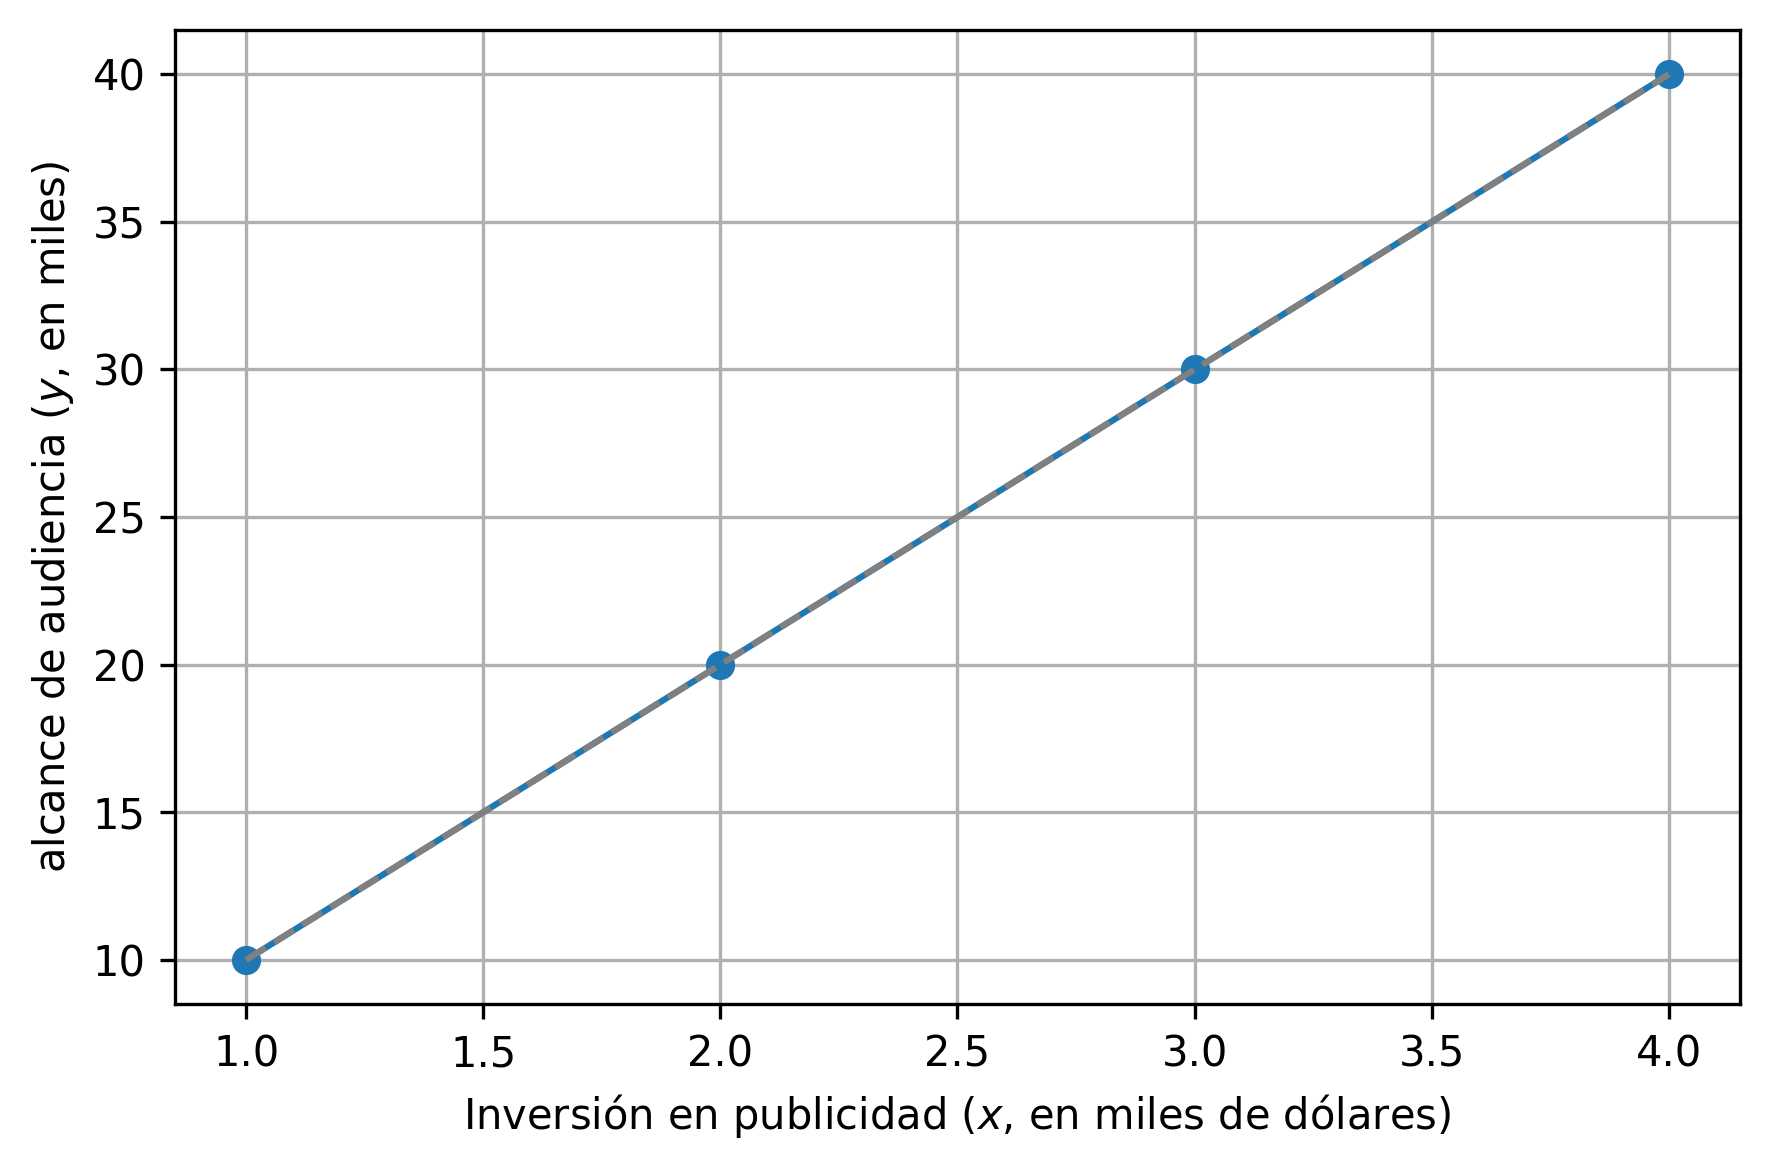
\includegraphics[keepaspectratio]{index_files/figure-pdf/cell-2-output-1.png}}

}

\end{figure}%

\paragraph{En general.}\label{en-general}

\begin{table}

{\caption{{Magnitudes directamente
proporcionales}{\label{tbl-mytable2}}}}

\begin{longtable}[]{@{}llll@{}}
\toprule\noalign{}
\(x\) & \(x_1\) & \(x_2\) & \(x_3\) \\
\midrule\noalign{}
\endhead
\bottomrule\noalign{}
\endlastfoot
\(y\) & \(y_1\) & \(y_2\) & \(y_3\) \\
\end{longtable}

{\noindent \emph{Note.} Elaboración propia}

\end{table}

donde se cumple que:

\[
\frac{x_1}{y_1} = \frac{x_2}{y_2} = \frac{x_3}{y_3} = k
\]

Lo que denotamos:

\[
\frac{x_i}{y_i} = k
\]

donde k es la constante de proporcionalidad directa. \(1 <= i < n\) ; i
pertenece a \(\mathbb{Z}\)

\paragraph{Funcion de proporcionalidad
directa.}\label{funcion-de-proporcionalidad-directa}

Se expresa mediante la función lineal homogénea:

\[
f(x) = kx
\]

donde \(f(x)\) representa la magnitud dependiente.

\paragraph{Magnitudes Inversamente
Proporcionales.}\label{magnitudes-inversamente-proporcionales}

Las magnitudes inversamente proporcionales son aquellas en las que el
incremento de una magnitud provoca una disminución proporcional en la
otra, por ejemplo:

\begin{table}

{\caption{{Relación entre Nivel de sensacionalismo en la noticia y
Credibilidad del medio}{\label{tbl-mytable2}}}}

\begin{longtable}[]{@{}lllll@{}}
\toprule\noalign{}
Nivel de sensacionalismo en la noticia & 20 & 10 & 5 & 2.5 \\
\midrule\noalign{}
\endhead
\bottomrule\noalign{}
\endlastfoot
Credibilidad del medio & 5 & 10 & 20 & 40 \\
\end{longtable}

{\noindent \emph{Note.} Elaboración propia}

\end{table}

Vemos que el Nivel de sensacionalismo en la noticia y la credibilidad
del medio son inversamente proporcionales. Luego:

\[
(\text{valor de sensacionalismo})*(\text{valor de credibilidad}) = (5)*(20) = (10)*(10) = (20)*(5) = (40)*(2.5) = Constante
\]

La constante de proporcionalidad inversa es:

\[
x \cdot y = 5 \cdot 20 = 100
\]

\paragraph{Gráficamente.}\label{gruxe1ficamente-1}

La gráfica de una función inversamente proporcional.

\begin{figure}[H]

\caption{Relación entre Nivel de sensacionalismo en la noticia y la
credibilidad del medio}

{\centering \pandocbounded{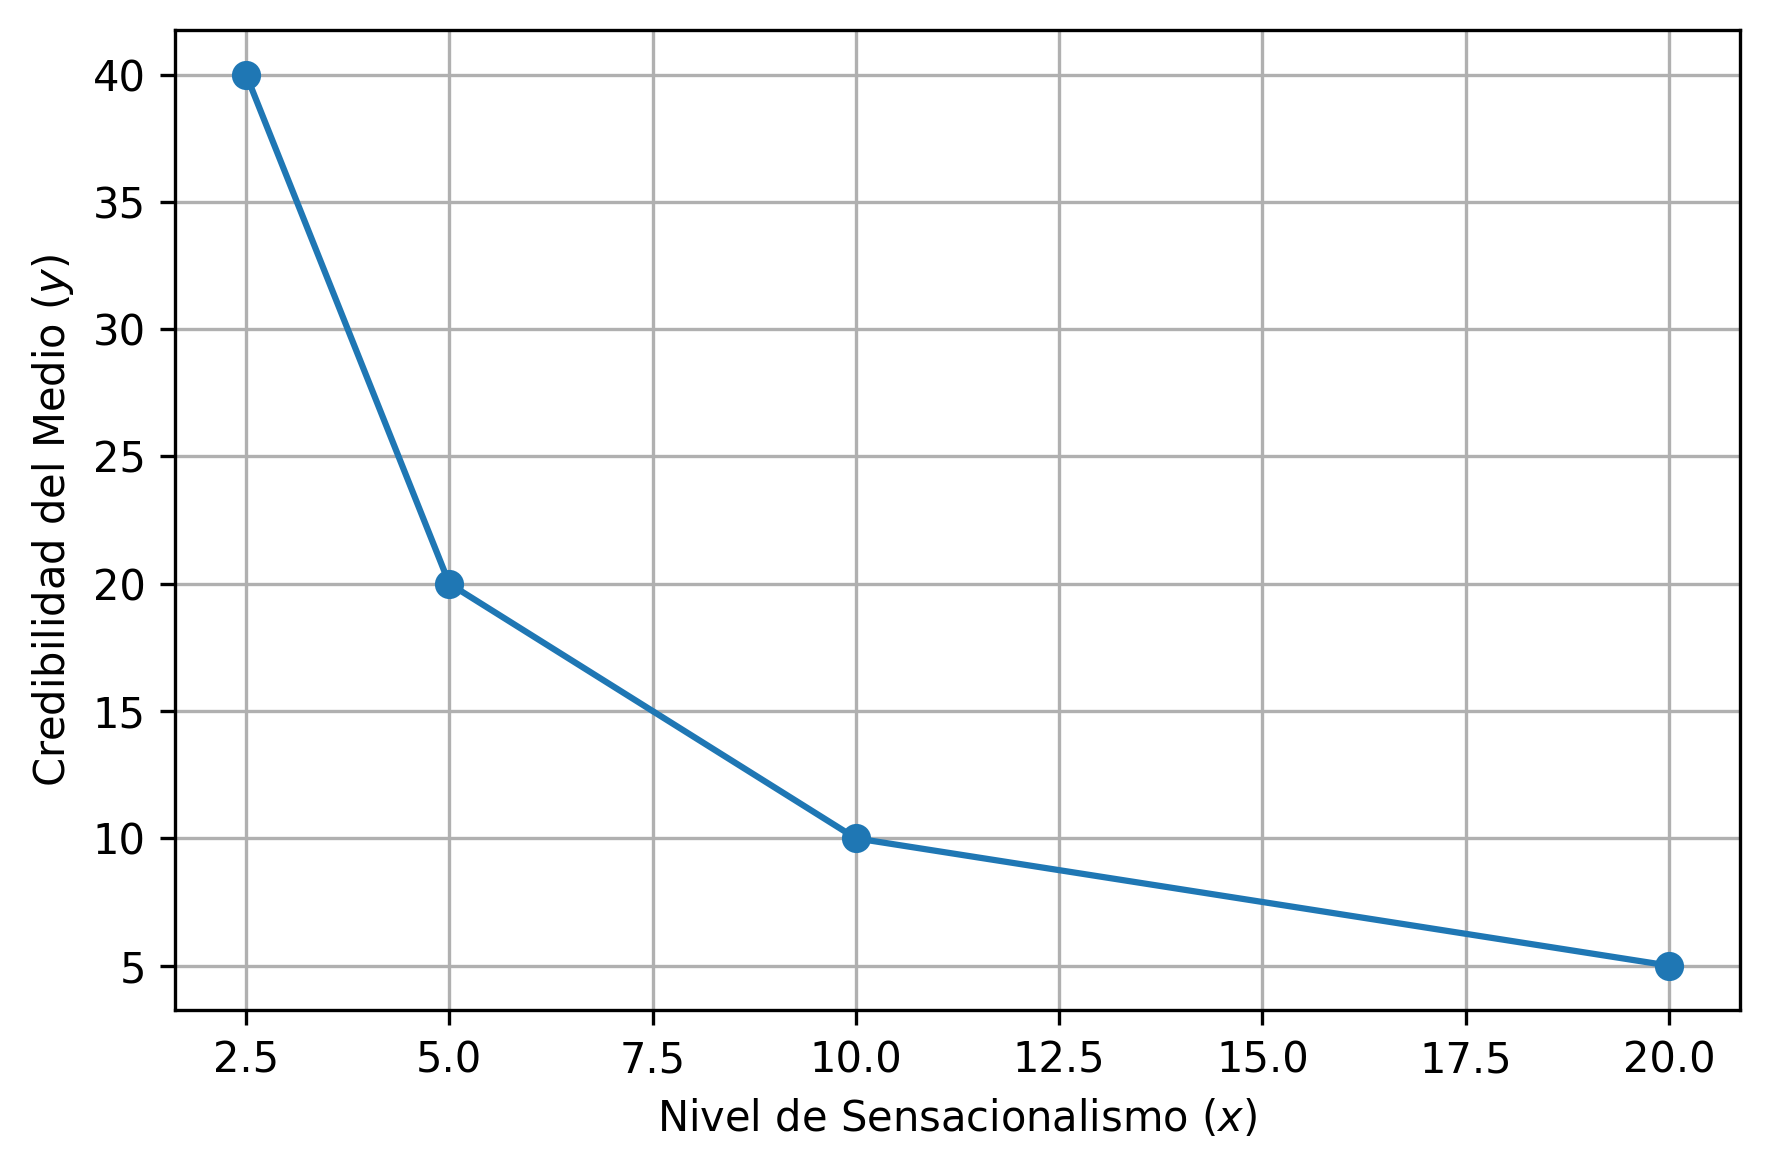
\includegraphics[keepaspectratio]{index_files/figure-pdf/cell-3-output-1.png}}

}

\end{figure}%

La gráfica muestra cómo a medida que aumenta el Nivel de
sensacionalismo, la credibilidad del medio disminuye, manteniendo una
relación inversa.

\paragraph{En general.}\label{en-general-1}

\begin{table}

{\caption{{Magnitudes inversamente
proporcionales}{\label{tbl-mytable2}}}}

\begin{longtable}[]{@{}llllll@{}}
\toprule\noalign{}
\(x\) & \(x_1\) & \(x_2\) & \(x_3\) & \ldots{} & \(x_n\) \\
\midrule\noalign{}
\endhead
\bottomrule\noalign{}
\endlastfoot
\(y\) & \(y_1\) & \(y_2\) & \(y_3\) & \ldots{} & \(y_n\) \\
\end{longtable}

{\noindent \emph{Note.} Elaboración propia}

\end{table}

donde se cumple que:

\[
x_1 \cdot y_1 = x_2 \cdot y_2 = x_3 \cdot y_3 = ... = X_n \cdot Y_n = k
\]

Lo que denotamos:

\[
y_i * x_i = k
\]

donde k es la constante de proporcionalidad inversa. \(1 <= i < n\) ; i
pertenece a \(\mathbb{Z}\)

\paragraph{Funcion de proporcionalidad
inversa.}\label{funcion-de-proporcionalidad-inversa}

La función de proporcionalidad inversa se expresa como:

\[
f(x) * x = k
\]

donde \(f(x)\) representa la magnitud dependiente.

\subsubsection{Propiedades}\label{propiedades}

Sean las magnitudes \(x\) e \(y\), entonces:

\begin{enumerate}
\item si $ x \text{ DP } y \Rightarrow y \text{ DP } x $
    \item $ x \text{ IP } y \Rightarrow y \text{ IP } x$
\item $ x \text{ IP } y \Leftrightarrow x \text{ DP } \left( \frac{1}{y} \right) $
\item $ x \text{ DP } y \Leftrightarrow x \text{ IP } \left( \frac{1}{y} \right) $
\item Si $ n \in \mathbb{Q} $, entonces:
\begin{itemize}
\item $ x \text{ DP } y \Leftrightarrow x^n \text{ DP } y^n $
\item $ x \text{ IP } y \Leftrightarrow x^n \text{ IP } y^n $
\end{itemize}
\end{enumerate}

\section{Aplicaciones de las Magnitudes
Proporcionales}\label{aplicaciones-de-las-magnitudes-proporcionales}

\subsection{Reparto Proporcional}\label{reparto-proporcional}

El reparto proporcional es un procedimiento matemático que distribuye
una cantidad total entre varias partes según una proporción determinada,
ya sea directa o inversa, en función de una variable de referencia. Este
concepto se divide en dos tipos principales: reparto directo e inverso.

\subsubsection{Reparto Directo}\label{reparto-directo}

El reparto directo se utiliza cuando se distribuye una cantidad total
entre varias partes de manera proporcional a sus magnitudes. Por
ejemplo, si se desea repartir un presupuesto de S/ 10,000 entre tres
departamentos directamente proporcional a de 2, 3 y 5, el reparto
proporcional se realiza de la siguiente manera:

\begin{align*}
&\text{Total a repartir: } 10\,000 \\
&\begin{cases}
2k = 2000 \\
3k = 3000 \\
5k = 5000 \\
\end{cases} \\
&2k + 3k + 5k = 10k = 10\,000 \\
&k = 1\,000
\end{align*}

\subsubsection{Reparto Inverso}\label{reparto-inverso}

El reparto inverso se aplica cuando se distribuye una cantidad total
entre varias partes de manera inversamente proporcional a sus
magnitudes. Por ejemplo, si se desea repartir un presupuesto de S/
180,000 entre tres departamentos inversamente proporcional a de 2, 3 y
6, el reparto proporcional inverso se realiza de la siguiente manera:

\begin{align*}
&\text{Total a repartir: } 180\,000 \\
&\begin{cases}
\frac{k}{2} = 90000 \\
\frac{k}{3} = 60000 \\
\frac{k}{6} = 30000 \\
\end{cases} \\
&\frac{k}{2} + \frac{k}{3} + \frac{k}{6} = 6k = 180\,000 \\
&k = 30\,000
\end{align*}

\subsection{Regla de Tres}\label{regla-de-tres}

\subsubsection{Regla de Tres Simple}\label{regla-de-tres-simple}

La regla de tres simple es un procedimiento matemático que permite
encontrar un cuarto valor desconocido a partir de tres valores
conocidos, en relaciones de proporcionalidad directa o inversa entre dos
magnitudes.

\begin{itemize}
\tightlist
\item
  \textbf{Regla de Tres Simple Directa}
\end{itemize}

\pandocbounded{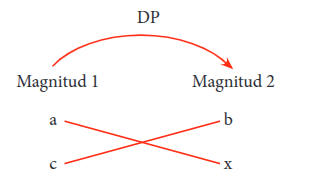
\includegraphics[keepaspectratio]{Screenshot_20250528_205612.png}}

Al ser Directamente Proporcional, se cumple:
\(\frac{Magnitud 1}{Magnitud 2} = k\)

De forma práctica, cuando sea regla de tres simple, directamente se
multiplica en aspa, igualando los resultados de la siguiente forma: \[
a \cdot x = b \cdot c
\]

\begin{itemize}
\tightlist
\item
  \textbf{Regla de Tres Simple Inversa}
\end{itemize}

\pandocbounded{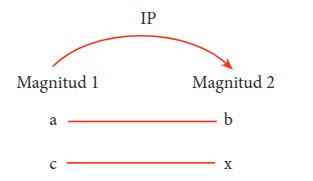
\includegraphics[keepaspectratio]{Screenshot_20250528_210518.png}}

Al ser Inversamente Proporcional, se cumple:
\(Magnitud 1 * Magnitud 2 = k\)

De forma práctica, cuando sea regla de tres simple inversa, se
multiplica de forma paralela, igualando los resultados de la siguiente
forma: \[
a \cdot b = c \cdot x
\]

\subsubsection{Regla de Tres Compuesta}\label{regla-de-tres-compuesta}

Es aquella operación matemática que se utiliza cuando en el problema
participan más de dos magnitudes.

\subsection{Porcentajes}\label{porcentajes}

El porcentaje es una expresión matemática que representa una relación
proporcional entre una parte y un todo, tomando como base el número
cien. Es una forma de expresar razones o fracciones en términos de ``por
cada cien'', facilitando la comparación y análisis de datos,
especialmente en contextos comunicacionales como encuestas, métricas de
audiencia o análisis de participación.

\[
\text{a por ciento de N} = a \% \text{de N} = \frac{a}{100} \cdot N
\]

Por ejemplo , si se desea calcular el 20\% de 150, se aplica la fórmula:
\[
\text{20\% de 150} = \frac{20}{100} \cdot 150 = 30
\]

Parte de un total como tanto por ciento

En general

\[
\frac{\text{Parte}}{\text{Total}} \cdot 100 \% = \frac{a}{b} \cdot 100 \%
\]

\subsubsection{Operaciones con
porcentajes}\label{operaciones-con-porcentajes}

\[
N = 100 \% N
\]

Ejmeplo

\[
32\%N + 48\%N = 80\%N
\]

\subsubsection{Aplicaciones de los
Porcentajes}\label{aplicaciones-de-los-porcentajes}

\begin{enumerate}
\def\labelenumi{\alph{enumi}.}
\tightlist
\item
  Descuentos sucesivos
\end{enumerate}

Para dos descuentos de a\% y b\%:

\[
\text{Descuento unico} = (a+b)-\frac{a \cdot b}{100}
\]

\begin{enumerate}
\def\labelenumi{\alph{enumi}.}
\setcounter{enumi}{1}
\tightlist
\item
  Aumentos sucesivos
\end{enumerate}

Para dos incrementos de a\% y b\%: \[  
\text{Aumento inicial} = (a+b)+\frac{a \cdot b}{100}
\]

\section{Ejemplos Aplicados a la Carrera de Periodismo y Ciencias de la
Comunicación}\label{ejemplos-aplicados-a-la-carrera-de-periodismo-y-ciencias-de-la-comunicaciuxf3n}

En las Ciencias de la Comunicación, las razones y proporciones son
herramientas importantes para optimizar estrategias, analizar datos y
diseñar campañas efectivas. A continuación, se presentan:

\subsection{Ejercicio 1: Regla de Tres Simple Directa para Calcular
Costo por
Impresión}\label{ejercicio-1-regla-de-tres-simple-directa-para-calcular-costo-por-impresiuxf3n}

\textbf{Problema:} Una campaña publicitaria en un medio digital cuesta
S/ 6,000 y genera 30,000 impresiones en redes sociales. Si se desea
calcular cuánto costaría alcanzar 45,000 impresiones, usa la regla de
tres simple directa para determinar el costo.

\textbf{Solución:}

La regla de tres simple directa se aplica porque el costo es
directamente proporcional al número de impresiones, es decir,
\(\frac{\text{Costo}}{\text{Impresiones}} = k\). La fórmula, según el
documento, es:

\[
a \cdot x = b \cdot c
\]

Donde: - \(a = 30,000\) (costo inicial) - \(b = 6,000\) (impresiones
iniciales) - \(c = 45,000\) (impresiones deseadas) - \(x\) = costo
desconocido

Configuramos la proporción:

\[
30,000 \cdot x = 6,000 \cdot 45,000
\]

Calculamos:

\[
30,000 \cdot x = 270,000,000
\]

\[
x = \frac{270,000,000}{30,000} = 9,000
\]

\textbf{Resultado:} El costo para alcanzar 45,000 impresiones es S/
9,000. Esta métrica ayuda a los comunicadores a planificar presupuestos
publicitarios.

\subsection{Ejercicio 2: Regla de Tres Simple Inversa para Tiempo de
Producción de
Contenido}\label{ejercicio-2-regla-de-tres-simple-inversa-para-tiempo-de-producciuxf3n-de-contenido}

\textbf{Problema:} Un equipo de 4 periodistas tarda 12 horas en producir
un reportaje investigativo. Si se aumenta el equipo a 6 periodistas,
¿cuánto tiempo tomará producir el mismo reportaje? Usa la regla de tres
simple inversa.

\textbf{Solución:}

La regla de tres simple inversa se aplica porque el tiempo es
inversamente proporcional al número de periodistas, es decir,
\(\text{Número de periodistas} \cdot \text{Tiempo} = k\). La fórmula,
según el documento, es:

\[
a \cdot b = c \cdot x
\]

Donde: - \(a = 4\) (número inicial de periodistas) - \(b = 12\) (horas
iniciales) - \(c = 6\) (nuevo número de periodistas) - \(x\) = tiempo
desconocido

Configuramos la proporción:

\[
4 \cdot 12 = 6 \cdot x
\]

\[
48 = 6 \cdot x
\]

\[
x = \frac{48}{6} = 8
\]

\textbf{Resultado:} Con 6 periodistas, el reportaje tomará 8 horas. Esta
aplicación es útil para gestionar recursos humanos en redacciones.

\subsection{Ejercicio 3: Reparto Proporcional Directo de un Presupuesto
Publicitario}\label{ejercicio-3-reparto-proporcional-directo-de-un-presupuesto-publicitario}

\textbf{Problema:} Un medio periodístico tiene un presupuesto de S/
15,000 para distribuir entre tres plataformas digitales (YouTube,
Instagram y TikTok) en proporción directa a sus suscriptores: 20,000,
30,000 y 50,000, respectivamente. Calcula cuánto le corresponde a cada
plataforma usando reparto proporcional directo.

\textbf{Solución:}

El reparto proporcional directo distribuye el total según las magnitudes
de los suscriptores. Según el documento, la fórmula es:

\[
\text{Monto por plataforma} = k \cdot \text{Suscriptores}
\]

Donde \(k\) es la constante de proporcionalidad, calculada como:

\[
k = \frac{\text{Presupuesto total}}{\text{Total de suscriptores}}
\]

\begin{enumerate}
\def\labelenumi{\arabic{enumi}.}
\tightlist
\item
  Calculamos el total de suscriptores:
\end{enumerate}

\[
20,000 + 30,000 + 50,000 = 100,000
\]

\begin{enumerate}
\def\labelenumi{\arabic{enumi}.}
\setcounter{enumi}{1}
\tightlist
\item
  Calculamos \(k\):
\end{enumerate}

\[
k = \frac{15,000}{100,000} = 0.15
\]

\begin{enumerate}
\def\labelenumi{\arabic{enumi}.}
\setcounter{enumi}{2}
\tightlist
\item
  Asignamos el monto a cada plataforma:
\end{enumerate}

\begin{itemize}
\tightlist
\item
  YouTube: \(20,000 \cdot 0.15 = S/ 3,000\)
\item
  Instagram: \(30,000 \cdot 0.15 = S/ 4,500\)
\item
  TikTok: \(50,000 \cdot 0.15 = S/ 7,500\)
\end{itemize}

\begin{enumerate}
\def\labelenumi{\arabic{enumi}.}
\setcounter{enumi}{3}
\tightlist
\item
  Verificamos la suma:
\end{enumerate}

\[
3,000 + 4,500 + 7,500 = 15,000
\]

\textbf{Resultado:} El presupuesto se distribuye como sigue: S/ 3,000
para YouTube, S/ 4,500 para Instagram y S/ 7,500 para TikTok. Esto
optimiza la inversión según el alcance de cada plataforma.

\subsection{Ejercicio 4: Reparto Proporcional Inverso para Asignación de
Espacios
Publicitarios}\label{ejercicio-4-reparto-proporcional-inverso-para-asignaciuxf3n-de-espacios-publicitarios}

\textbf{Problema:} Una revista digital tiene S/ 12,000 para pagar
espacios publicitarios en tres secciones, y desea distribuir el
presupuesto inversamente proporcional a la cantidad de anuncios ya
publicados en cada una: 2, 4 y 6 anuncios, respectivamente. Calcula
cuánto le corresponde a cada sección usando reparto proporcional
inverso.

\textbf{Solución:}

El reparto proporcional inverso distribuye el total inversamente a las
magnitudes. Según el documento, la fórmula es:

\[
\text{Monto por sección} = \frac{k}{\text{Número de anuncios}}
\]

Y la suma de los términos inversos satisface:

\[
\frac{k}{a_1} + \frac{k}{a_2} + \frac{k}{a_3} = \text{Presupuesto total}
\]

Donde: - \(a_1 = 2\), \(a_2 = 4\), \(a_3 = 6\) - Presupuesto total =
12,000

\begin{enumerate}
\def\labelenumi{\arabic{enumi}.}
\tightlist
\item
  Calculamos la suma de los inversos:
\end{enumerate}

\[
\frac{1}{2} + \frac{1}{4} + \frac{1}{6} = 0.5 + 0.25 + 0.1667 = 0.9167
\]

\begin{enumerate}
\def\labelenumi{\arabic{enumi}.}
\setcounter{enumi}{1}
\tightlist
\item
  Calculamos \(k\):
\end{enumerate}

\[
k \cdot 0.9167 = 12,000
\]

\[
k = \frac{12,000}{0.9167} \approx 13,090.91
\]

\begin{enumerate}
\def\labelenumi{\arabic{enumi}.}
\setcounter{enumi}{2}
\tightlist
\item
  Asignamos el monto a cada sección:
\end{enumerate}

\begin{itemize}
\tightlist
\item
  Sección 1: \(\frac{13,090.91}{2} \approx S/ 6,545.46\)
\item
  Sección 2: \(\frac{13,090.91}{4} \approx S/ 3,272.73\)
\item
  Sección 3: \(\frac{13,090.91}{6} \approx S/ 2,181.82\)
\end{itemize}

\begin{enumerate}
\def\labelenumi{\arabic{enumi}.}
\setcounter{enumi}{3}
\tightlist
\item
  Verificamos la suma (aproximada por redondeo):
\end{enumerate}

\[
6,545.46 + 3,272.73 + 2,181.82 \approx 12,000
\]

\textbf{Resultado:} El presupuesto se distribuye aproximadamente como:
S/ 6,545.46 para la sección con 2 anuncios, S/ 3,272.73 para la sección
con 4 anuncios y S/ 2,181.82 para la sección con 6 anuncios. Esto
prioriza secciones con menos saturación publicitaria.

\subsection{Ejercicio 5: Cálculo de Porcentaje de Participación en una
Encuesta}\label{ejercicio-5-cuxe1lculo-de-porcentaje-de-participaciuxf3n-en-una-encuesta}

\textbf{Problema:} En una encuesta realizada por un medio periodístico
sobre preferencias electorales, 240 de 800 encuestados apoyan a un
candidato. Calcula el porcentaje de apoyo al candidato.

\textbf{Solución:}

El porcentaje se calcula como la relación entre la parte y el total,
multiplicado por 100, según la fórmula del documento:

\[
\text{Porcentaje} = \frac{\text{Parte}}{\text{Total}} \cdot 100
\]

Sustituyendo los valores:

\[
\text{Porcentaje} = \frac{240}{800} \cdot 100 = 30\%
\]

\textbf{Resultado:} El 30\% de los encuestados apoya al candidato. Este
porcentaje es clave para reportar tendencias electorales y analizar el
impacto de la cobertura mediática.

\section{Conclusiones y
Recomendaciones}\label{conclusiones-y-recomendaciones}

La regla de tres simple, el reparto proporcional y los porcentajes son
herramientas esenciales en las ciencias de la comunicación, ya que
facilitan la gestión eficiente de recursos, el análisis de audiencias y
la planificación de estrategias mediáticas. Su aplicación permite a los
comunicadores interpretar métricas, asignar presupuestos equitativamente
y optimizar procesos de producción, conectando la teoría matemática con
las demandas prácticas de la profesión.

Se recomienda integrar estas herramientas en los programas académicos de
la escuela profesional, con un enfoque en ejercicios prácticos basados
en escenarios reales, como la distribución de publicidad o la evaluación
de encuestas. Asimismo, se sugiere crear recursos digitales interactivos
que simplifiquen el uso de estas técnicas, fortaleciendo las
competencias cuantitativas de los profesionales y mejorando la precisión
en la toma de decisiones estratégicas.

\section{Bibliografía y
referencias}\label{bibliografuxeda-y-referencias}

Arican, M., \& Kiymaz, Y. (2022). Investigating preservice mathematics
teachers' definitions, formulas, and graphs of directly and inversely
proportional relationships. \emph{The Mathematics Enthusiast, 19}(2),
5--16.
https://scispace.com/papers/investigating-preservice-mathematics-teachers-definitions-2oii9y83

D'Amore, B. (2005a). \emph{Didáctica de la matemática: Ideas para una
teoría}. Narcea Ediciones.

D'Amore, B. (2005b). \emph{Matemáticas y su didáctica}. Paidós.

Euclides. (ca. 300 a.C./1908). \emph{Elementos} (T. L. Heath, Trans.).
Cambridge University Press. (Original work published ca. 300 BCE)

Gómez, A. (2011). \emph{Matemáticas aplicadas a las ciencias sociales
I}. McGraw-Hill.
https://www.mheducation.es/bcv/guide/capitulo/8448186618.pdf

Gómez, J. (2011). \emph{Matemáticas aplicadas a las ciencias sociales}.
Pirámide.

Heath, T. L. (1908). \emph{The thirteen books of Euclid's Elements}
(Vol. 2). Cambridge University Press.

López Pan, F., \& Vicente, M. (2016). \emph{Análisis de contenido en
comunicación}. Síntesis.

Martínez, P., \& Piñuel, J. L. (2011). \emph{Métricas de audiencia}.
Gedisa.

Pérez Ruiz, L., \& Domínguez, M. (2015). \emph{Publicidad y
comunicación}. ESIC.

Rico, L. (2008a). \emph{Didáctica de las matemáticas}. Morata.

Rico, L. (2008b). \emph{Educación matemática: Una visión de conjunto}.
Síntesis.

Rodríguez Morales, J. (2012). \emph{Diseño gráfico y comunicación
visual}. Trillas.

Vitruvio. (ca. 15 a.C./1999). \emph{De Architectura} (I. D. Rowland,
Trans.). Cambridge University Press. (Original work published ca. 15
BCE)

Williams, K. (2019). \emph{Proporciones en la arquitectura
renacentista}. Routledge.






\end{document}
